	\documentclass[10pt]{scrartcl}

\usepackage[utf8]{inputenc}
\usepackage{tabularx}
\usepackage[ngerman]{babel}
\usepackage[automark]{scrpage2}
\usepackage{amsmath,amssymb,amstext}
\usepackage[]{color}
\usepackage[]{enumerate}
\usepackage{graphicx}
\usepackage{lastpage}
\usepackage[perpage,para,symbol*]{footmisc}
\usepackage{listings} 
\usepackage[pdfborder={0 0 0},colorlinks=false]{hyperref}
\usepackage[numbers,square]{natbib}

\lstset{numbers=left, numberstyle=\tiny, numbersep=5pt, breaklines=true, showstringspaces=false} 

%changehere
\def\titletext{Praktikum 1 : DGL}
\def\titletextshort{Praktikum 1}
\author{André Harms, Oliver Steenbuck}

\title{\titletext}

%changehere Datum der Übung
\date{02.11.2011}

\pagestyle{scrheadings}
%changehere
\ihead{MT, Pareigis}
\ifoot{Generiert am:\\ \today}

\cfoot{Oliver Steenbuck \\ Andre Harms}

\ohead[]{\titletextshort}
\ofoot[]{{\thepage} / \pageref{LastPage}}

\setlength{\parindent}{0.0in}
\setlength{\parskip}{0.1in}

\begin{document}
\maketitle

\setcounter{tocdepth}{3}
\tableofcontents
%\bibpunct{(}{)}{;}{n}{,}{,}

\section{Steife Differentialgleichungen}
	\subsection{Simulink/Analogrechner}
	
	\begin{figure}[htbp]
	\centering
		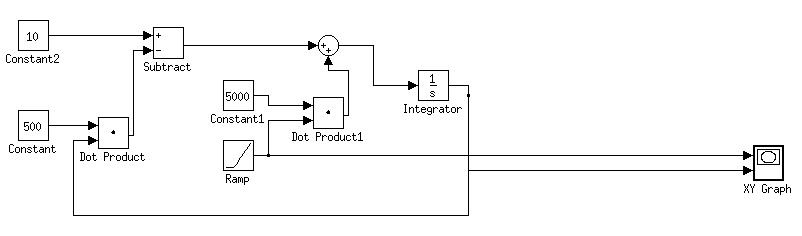
\includegraphics[scale=0.5]{simulink_aufg1_a}
	\caption{abbildung 1}
	\label{fig:abb1}
	\end{figure}

	\subsection{Iterationsgleichungen}
		\subsubsection{Euler (expl)}
		
		\subsubsection{Euler (impl)}
		
		\subsubsection{Runge-Kutta 2}
		
	\subsection{Matlab Programme}
		\subsubsection{Euler (expl)}
			\lstinputlisting[label=code_euler_expl,caption=Explizites Euler-Verfahren, language=Matlab]{euler_expl.m}
		
		\subsubsection{Euler (impl)}
				\lstinputlisting[label=code_euler_impl,caption=Implizites Euler-Verfahren, language=Matlab]{euler_impl.m}
		
		\subsubsection{Runge\-Kutta}
				\lstinputlisting[label=code_runge_kutta,caption=Runge Kutta, language=Matlab]{rk2.m}
		
		\subsubsection{stiff}		
		
	\subsection{Ergebnisausdrucke}	
		
	\subsection{Interpretation der Ergebnisse}		
		

\section{Van-der-Pol-DGL}
	\subsection{Simulink/Analogrechner}
	\begin{figure}[htbp]
	\centering
		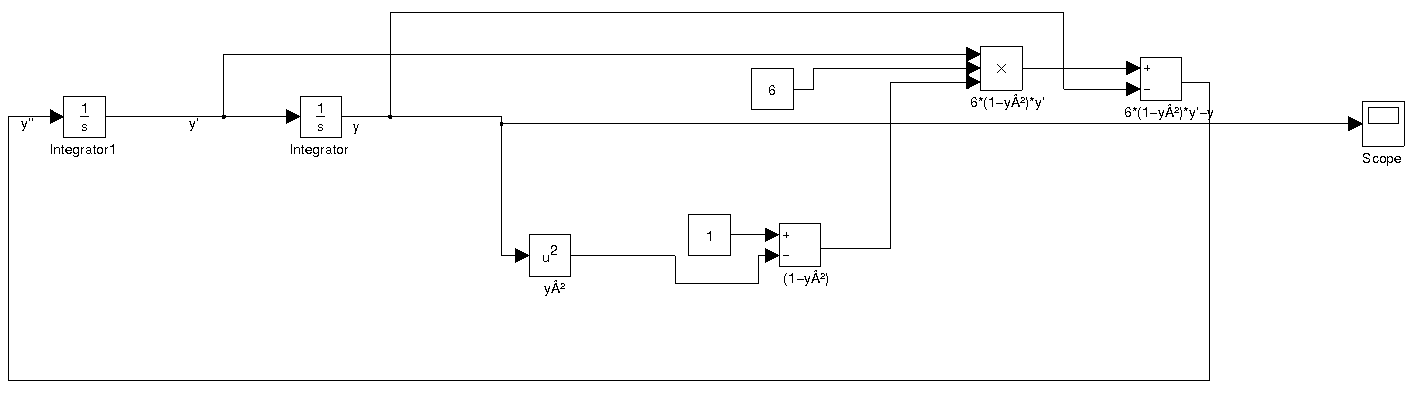
\includegraphics[scale=0.4]{aufg2_a_simulink}
	\caption{Simulink-Schaltbild Van-der-Pol-DGL}
	\label{fig:simulinkAufg2}
	\end{figure}	
	
	\subsection{Zu DGL 1 Ordnung transformierte DGL}
	
	\subsection{Iterationsgleichungen}
		\subsubsection{Euler (expl)}	
	
		\subsubsection{Runge-Kutta 2}	
		
	\subsection{Ergebnisausdrucke}	
		
	\subsection{Interpretation der Ergebnisse}	
	
\section{Lorenz-Attraktor mit RK 2}	
	\subsection{Simulink/Analogrechner}
	
	\subsection{Iterationsgleichungen}
		\subsubsection{Runge-Kutta 2}

	\subsection{Matlab Programme}
		\subsubsection{Lorenz}			

	\subsection{Ergebnisausdrucke}	
		
	\subsection{Interpretation der Ergebnisse}				

\end{document}

